\documentclass[runningheads]{llncs}

\usepackage{iftex}
\ifPDFTeX
  \PackageError{main_vi}{Tài liệu này phải được biên dịch bằng XeLaTeX}{}
\else
  \usepackage{fontspec}
  \setmainfont{DejaVu Serif}
\fi
\usepackage{polyglossia}
\setdefaultlanguage{vietnamese}
\usepackage{amsmath,amssymb}
\usepackage{booktabs}
\usepackage{graphicx}
\usepackage{xcolor}
\usepackage{hyperref}
\IfFileExists{algorithm.sty}{%
  \usepackage{algorithm}%
}{%
  \usepackage{float}%
  \newfloat{algorithm}{tbp}{loa}%
  \floatname{algorithm}{Thuật toán}%
}
\IfFileExists{algpseudocode.sty}{%
  \usepackage{algpseudocode}%
}{%
  \newcounter{algline}%
  \newenvironment{algorithmic}[1][1]{%
    \setcounter{algline}{0}%
    \begin{list}{}{\setlength{\leftmargin}{3.2em}\setlength{\labelwidth}{2.4em}%
      \setlength{\labelsep}{0.6em}\setlength{\itemsep}{0.15ex}\setlength{\parsep}{0pt}%
      \setlength{\topsep}{0.2ex}}\small\normalfont}{\end{list}}%
  \newcommand{\algitem}{\stepcounter{algline}%
    \item[{\makebox[2.4em][r]{\thealgline:}}]}%
  \newcommand{\State}{\algitem}%
  \newcommand{\Statex}{\item[]}%
  \newcommand{\Require}{\item[\textbf{Đầu vào:}]}%
  \newcommand{\Ensure}{\item[\textbf{Đầu ra:}]}%
  \newcommand{\For}[1]{\algitem\textbf{với mỗi}~##1~\textbf{thực hiện}}%
  \newcommand{\EndFor}{\algitem\textbf{kết thúc vòng lặp}}%
  \newcommand{\If}[1]{\algitem\textbf{nếu}~##1~\textbf{thì}}%
  \newcommand{\Else}{\algitem\textbf{ngược lại}}%
  \newcommand{\EndIf}{\algitem\textbf{kết thúc nếu}}%
  \newcommand{\Function}[2]{\algitem\textbf{hàm}~\textproc{##1}(##2)}%
  \newcommand{\EndFunction}{\algitem\textbf{kết thúc hàm}}%
  \newcommand{\Call}[2]{\textproc{##1}(##2)}%
  \newcommand{\Return}{\textbf{trả về}~}%
  \newcommand{\Comment}[1]{\hfill{\footnotesize\(\triangleright\)~##1}}%
  \providecommand{\textproc}[1]{\textsc{##1}}%
}
\usepackage{placeins}
\renewcommand\UrlFont{\color{blue}\rmfamily}
\urlstyle{rm}
\graphicspath{{figures/}}
\emergencystretch=1.5em

\begin{document}

\title{Kiểm thử sức chịu đựng của phân cụm có cổng tích và xếp hạng ưu tiên
bị chặn cho các báo cáo cứu hộ lũ: Nghiên cứu tổng hợp}
\titlerunning{Kiểm thử phân cụm và xếp hạng báo cáo cứu hộ lũ}

\author{Thanh-Trong Nguyen\inst{1}\orcidID{0009-0007-6976-5131}\thanks{Tác giả liên hệ.} \and
Ngoc-Anh Le\inst{1}\orcidID{0009-0006-7453-1009} \and
Nhu-Quynh Nguyen\inst{1}\orcidID{0009-0008-7396-697X} \and
Tuong-Hung Cao\inst{1}\orcidID{0009-0003-5886-2666} \and
Hung-Thinh Ngo\inst{1}\orcidID{0009-0004-8668-4462} \and
Thanh-Khoa Nguyen\inst{1}\orcidID{0000-0002-0012-1158}}
\authorrunning{T.-T. Nguyen và cộng sự}
\institute{Khoa Công nghệ Thông tin và Truyền thông,
Trường Đại học Cần Thơ, Cần Thơ, Việt Nam\\
\email{ngthtrong204@gmail.com}}

\maketitle

\begin{abstract}
Các luồng thông tin về lũ phục vụ tác nghiệp thường chứa báo cáo trùng lặp,
không đầy đủ và có tính đối kháng, trong khi phân cụm và điểm ưu tiên thường
được đánh giá mà không đo lường hệ quả lập lịch. Chúng tôi kiểm toán một
đường ống xử lý theo lô, đóng khi thiếu dữ liệu, trong đó các báo cáo quan
sát được tạo thành một đồ thị thưa, báo cáo chưa phân giải được chuyển sang
kiểm duyệt, các họ trùng lặp cung cấp đầu vào cho một điểm bị chặn, còn chân
trị chỉ dành cho đánh giá được nối sau khi lập lịch các cụm dự đoán. Bộ kiểm
thử phân cụm gồm 80 lần chạy từ bộ sinh 3.0.0: Louvain cộng có ARI trung
bình $0.9191$, Leiden tích $0.9165$ và Louvain tích $0.9072$. Hiệu của tích
so với cộng được hiệu chỉnh độc lập là $-0.0118$ (KTC bootstrap 95\%
$[-0.0226,-0.0024]$), nhưng kiểm định hiệu chỉnh Holm không có ý nghĩa
($p=.2560$). So sánh cùng mật độ đảo chiều ước lượng điểm nhưng cũng không
kết luận được. Trong một bó Candidate-4.1 riêng, điểm sửa đổi có NDCG@5
$0.6669$ so với $0.6763$ của bộ so sánh ngẫu nhiên và không cho thấy ưu thế
đồng chỉnh tổng quát; các bản sao chính xác là bất biến, nhưng các chiến dịch
phối hợp có độ tin cậy cao vẫn là một dạng thất bại. Kết quả điều phối cũng
không cho thấy lợi ích tổng quát so với điểm cũ và có chi phí rõ rệt so với
chiến lược gần nhất trước. Đây là các chẩn đoán tổng hợp, trong cùng một bộ
sinh: tính bị chặn và độ chính xác phân cụm không chứng minh được tính xác
thực của nguồn, tính hợp lệ chính sách, lợi ích thực địa hay mức sẵn sàng
triển khai.
\keywords{Cứu hộ lũ \and Phân cụm đồ thị \and Kiểm thử tổng hợp \and
Xếp hạng ưu tiên \and Kết quả âm.}
\end{abstract}

\section{Giới thiệu và công trình liên quan}

Trong tình huống khẩn cấp, các luồng thông tin khủng hoảng trộn lẫn nhiều
báo cáo lặp lại về một sự kiện, các sự kiện khác nhau nhưng ở gần nhau, các
trường bị thiếu và nhiễu không liên quan. Nghiên cứu về cảm biến xã hội và
trích xuất sự kiện xử lý bài toán về quy mô, xác minh và nhận dạng sự kiện
\cite{sakaki2010earthquake}. CrisisMMD và FloodNet cung cấp các phương thức
thảm họa hữu ích, dù FloodNet là bộ dữ liệu hiểu cảnh sau lũ từ ảnh trên
không, chứ không phải luồng báo cáo đa phương thức
\cite{alam2018crisismmd,rahnemoonfar2021floodnet}. Những nguồn này không
đồng thời cung cấp liên kết sự cố vật lý, mức ưu tiên cứu hộ và kết quả điều
phối ngoài thực địa.

\paragraph{Cảm biến xã hội và trích xuất sự kiện.}
Người dùng mạng xã hội có thể hoạt động như các cảm biến thời gian thực
\cite{sakaki2010earthquake}, nhưng đầu ra thường là phát hiện hoặc phân
loại sự kiện, thay vì hệ quả của việc điều một nguồn lực thực địa đến một sự
cố được dự đoán.

\paragraph{Hợp nhất và phân cụm.}
Phát hiện cộng đồng trên đồ thị bằng Louvain hoặc Leiden
\cite{blondel2008louvain,traag2019leiden}, cùng các phương pháp mật độ như
DBSCAN và HDBSCAN \cite{ester1996dbscan}, là các cơ chế hợp nhất khả dĩ.
Các số hạng tích không gian--phạm vi xuất hiện trong bộ lọc song phương
\cite{tomasi1998bilateral}; chúng tôi điều chỉnh cấu trúc đó cho đồ thị tích,
đồng thời kiểm thử chính xác cổng và các chặn của nó trong bài này.

\paragraph{Hậu cần nhân đạo và điều phối.}
Các mô hình định tuyến cứu trợ bộc lộ sự cạnh tranh giữa các mục tiêu công
bằng, hiệu lực và hiệu quả \cite{gralla2014review}. Chúng tôi dùng góc nhìn
này để thúc đẩy một phép xếp hạng ưu tiên bị chặn, nhưng tính bị chặn không
đồng nghĩa với một chính sách cứu hộ đã được chuyên gia xác nhận. Khoảng
trống then chốt là sự lan truyền của các lỗi tách, gộp và nhiễu vào một bộ
lập lịch không thể truy cập chân trị sự cố.

Chúng tôi giải quyết các khoảng trống đó bằng một đường ống xử lý theo lô,
đóng khi thiếu dữ liệu: báo cáo có vị trí và thời gian quan sát được đi vào
đồ thị thưa, báo cáo chưa đầy đủ chuyển sang kiểm duyệt thủ công, các họ
trùng lặp cung cấp đầu vào cho xếp hạng bị chặn, và chân trị chỉ dành cho
đánh giá được nối sau khi lập lịch các cụm dự đoán. Ba câu hỏi là: (RQ1)
việc chọn độc lập thành phần tích có cải thiện phân cụm so với thành phần
cộng không? (RQ2) điểm có xét trùng lặp có đồng chỉnh với lợi ích được sinh
độc lập dưới các kiểm thử sức chịu đựng cấp báo cáo không? (RQ3) lỗi tách,
gộp và nhiễu của cụm dự đoán lan truyền vào điều phối như thế nào? Hai bó
hiện vật được tách biệt rõ ràng trong các câu hỏi này.

Các đóng góp gồm: (i) đường ống chỉ dùng thông tin quan sát được, với ranh
giới kiểm duyệt và đánh giá rõ ràng; (ii) các phát biểu ngưỡng có thể kiểm
toán và một điểm đề xuất có xét trùng lặp; và (iii) báo cáo chẩn đoán ghép
phân cụm, xếp hạng, điều phối và các kết quả bất lợi. Giá trị khoa học
chính nằm ở các kết quả âm và kết quả biên có thể kiểm toán: những lỗi lan
truyền và lỗ hổng đối kháng vốn bị che khuất trong chuẩn đánh giá chỉ dựa
trên độ chính xác được làm rõ và định lượng. Bằng chứng vẫn là tổng hợp và
chỉ trong cùng bộ sinh, nên hiện vật này không phải chính sách cứu hộ đã
được xác nhận.

\section{Đường ống quan sát được và phương pháp}

Hình~\ref{fig:pipeline} cố định ranh giới thông tin. Các trường nhìn thấy
khi tiếp nhận đi qua bước xây dựng đồ thị, xếp hạng và bộ lập lịch theo lô.
Báo cáo thiếu vị trí hoặc thời gian sự kiện được chuyển sang kiểm duyệt.
Danh tính sự cố, lợi ích, hạn chót và mức thiệt hại được lưu riêng và chỉ
được nối sau khi đã có lịch.

\begin{figure}[t]
\centering
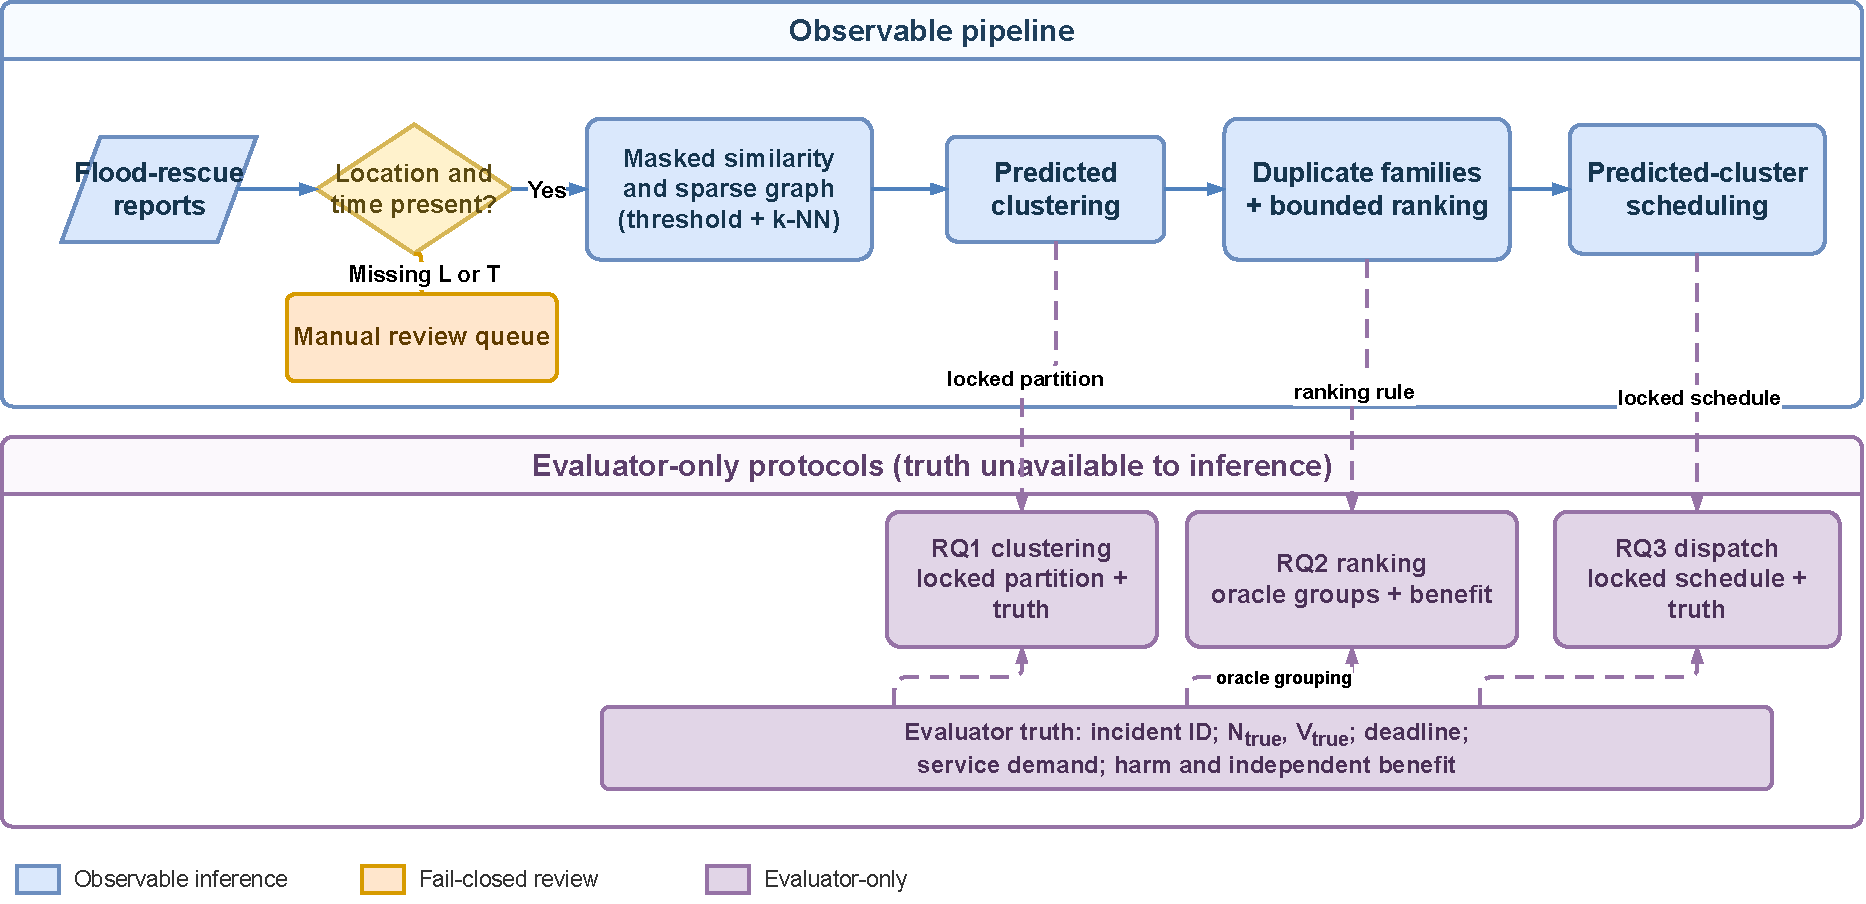
\includegraphics[width=\textwidth]{pipeline_v2.pdf}
\caption{Đường ống quan sát được (đường liền), nhánh kiểm duyệt thủ công
(màu cam) và phép nối chân trị chỉ dành cho đánh giá (nét đứt). Bộ lập lịch
chỉ nhận các cụm dự đoán, không bao giờ nhận chân trị sự cố.}
\label{fig:pipeline}
\end{figure}

Thuật toán~\ref{alg:pipeline} viết lại đường suy luận thực thi dưới dạng mã
giả: cổng tiếp nhận và chuyển sang kiểm duyệt (Mục~2.1), xây dựng đồ thị
tương tự và phân cụm (Mục~2.2), chấm điểm cụm có xét trùng lặp (Mục~2.3,
chi tiết trong Thuật toán~\ref{alg:priority}) và lập lịch. Phép nối chân trị
chỉ dành cho đánh giá được mô tả sau thuật toán và không bao giờ là đầu vào
của đường suy luận.

\begin{algorithm}[!tbp]
\caption{Đường ống báo cáo đóng khi thiếu dữ liệu (Hình~\ref{fig:pipeline})}
\label{alg:pipeline}
\begin{algorithmic}[1]
\Require Báo cáo $R=\{r_i\}$; các thang kernel $\sigma,\tau_t,\tau_F,\tau_E$;
trọng số $\beta,\gamma$ (và $\alpha$ cho thành phần cộng); phân vị $q$;
giới hạn láng giềng $k$; độ phân giải Louvain/Leiden $\rho$; thành phần
$m\in\{\text{tích},\text{cộng}\}$
\Ensure Lịch điều phối $S$; thuật toán không đọc nhãn danh tính sự cố, lợi
ích, hạn chót hay thiệt hại
\State $R_{\rm obs}\gets\emptyset$; $R_{\rm review}\gets\emptyset$
\For{mỗi báo cáo $r_i\in R$}
    \State $a_i\gets\mathbf{1}\{L_i,T_i\text{ quan sát được}\}$
    \If{$a_i=0$}
        \State $R_{\rm review}\gets R_{\rm review}\cup\{r_i\}$
        \Comment{nhánh kiểm duyệt thủ công}
    \Else
        \State $R_{\rm obs}\gets R_{\rm obs}\cup\{r_i\}$
    \EndIf
\EndFor
\State Tính $n_i^{\rm corrob}$ từ các payload quan sát duy nhất trong toàn bộ
$R_{\rm obs}$, rồi đặt
\Statex \hspace{1em}$Q_i\gets\operatorname{sigmoid}\bigl(b_0+b_1\mathbf{1}\{\text{image}_i\}
 +b_2\log(1+n_i^{\rm corrob})\bigr)$ cho mọi $r_i\in R_{\rm obs}$
\State $E_0\gets$ \Call{BuildSimilarityEdges}{$R_{\rm obs},m,\sigma,\tau_t,\tau_F,\tau_E,\alpha,\beta,\gamma$}
\State $\theta\gets$ phân vị $q$ của các trọng số khác không trong $E_0$
\State $E_\theta\gets\{(i,j,w_{ij})\in E_0:w_{ij}>\theta\}$
\State $E\gets E_\theta\cup\text{(các cạnh top-}k\text{ theo từng đầu mút trong }E_\theta\text{), đối xứng hóa bằng OR}$
\State $\mathcal{G}\gets(R_{\rm obs},E)$
\State $\mathcal{C}\gets$ Louvain/Leiden$(\mathcal{G},\rho)$
\Comment{cụm dự đoán, không dùng chân trị}
\For{mỗi cụm dự đoán $C_k\in\mathcal{C}$}
    \State $P_k\gets$ \Call{PriorityScore}{$C_k$}
\EndFor
\State $S\gets$ Scheduler$(\{(C_k,P_k):C_k\in\mathcal{C}\})$
\Comment{bộ lập lịch chỉ thấy cụm dự đoán và $P_k$}
\State \Return $S$
\end{algorithmic}
\end{algorithm}

\FloatBarrier

Sau khi cố định $S$, bộ đánh giá ngoại tuyến có thể nối $S$ và
$R_{\rm review}$ với danh tính sự cố, lợi ích, hạn chót và nhãn thiệt hại để
tính ARI, NDCG@5 và các kết quả điều phối. Nhánh nét đứt này không có trong
thuật toán suy luận. Trong các hiện vật hiện tại, lược đồ lõi yêu cầu vị trí
và thời gian sự kiện, vì vậy nhánh kiểm duyệt thủ công là ranh giới thiết kế
đóng khi thiếu dữ liệu, chứ chưa phải điều kiện thiếu dữ liệu được đánh giá
thực nghiệm.

\subsection{Thuộc tính báo cáo và dữ liệu thiếu}

Mỗi báo cáo được biểu diễn bởi bộ
\[
r_i=(L_i,T_i,F_i,E_i,N_i,V_i,Q_i),
\]
trong đó $L_i$ là vị trí GPS và $T_i$ là dấu thời gian báo cáo quan sát được
(``created\_at''). Bằng chứng lũ $F_i$ và bằng chứng khẩn cấp $E_i$ thuộc
$[0,1]$; $N_i\in\mathbb{Z}_{\geq0}$ là số người mắc kẹt được báo cáo;
$V_i\geq0$ là giá trị bằng chứng về tính dễ tổn thương; còn
$Q_i\in[0,1]$ là heuristic về nguồn gốc/độ tin cậy. $Q_i$ không phải xác
suất chân lý đã hiệu chỉnh. Cài đặt cũng mang các trường hỗ trợ quan sát được
như có ảnh, loại nguồn, tỉnh và cờ thiếu trường; chúng hỗ trợ $Q_i$ và dấu
vân tay trùng lặp nhưng không phải nhãn ẩn bổ sung.

Điểm $Q_i$ được tính từ việc có ảnh và số payload quan sát gần đó có khả năng
đối chứng (đếm theo định danh payload duy nhất), theo heuristic
\[
\begin{aligned}
Q_i&=\operatorname{sigmoid}\!\left(b_0+b_1\mathbf{1}\{\text{image}_i\}
 +b_2\log(1+n_i^{\rm corrob})\right),\\[-1mm]
(b_0,b_1,b_2)&=(-.2,1.4,.9).
\end{aligned}
\]
Ở đây $\operatorname{sigmoid}(x)=(1+e^{-x})^{-1}$. Đây là quy tắc đường
ống, không phải mô hình chân lý đã hiệu chỉnh. Không giả định có dấu thời
gian tiếp nhận độc lập hay họ nguồn độc lập.

Theo bài toán kernel với biến thiếu nói chung~\cite{smola2005missing},
chúng tôi dùng cấu trúc đóng khi thiếu dữ liệu sau. Chỉ báo tiếp nhận là
$a_i=\mathbf{1}\{L_i,T_i\text{ quan sát được}\}$. Do đó $a_i a_j=0$ ngăn
một cạnh liên quan đến báo cáo không xác định được khoảng cách địa lý hoặc
thời gian; báo cáo đó đi theo nhánh kiểm duyệt thủ công. $F_i$ hoặc $E_i$
thiếu không được gán bằng 0: gọi $I_F(i,j),I_E(i,j)$ là các chỉ báo hai báo
cáo cùng quan sát trường tương ứng và đặt $m_{ij}=I_F(i,j)+I_E(i,j)$; khi đó
\[
C_{ij}=\frac{m_{ij}}{2}\exp\!\left[-I_F(i,j)\frac{|F_i-F_j|}{\tau_F}
-I_E(i,j)\frac{|E_i-E_j|}{\tau_E}\right],
\quad C_{ij}=0\ \text{nếu }m_{ij}=0.
\]
Khi $m_{ij}=2$, cả hai trường ngữ cảnh được dùng; khi $m_{ij}=1$, độ tương
đồng ngữ cảnh cực đại bị giảm còn $1/2$; và khi $m_{ij}=0$, không suy ra
được sự đồng thuận ngữ cảnh. Trong hiện vật 80 lần chạy hiện tại, mọi báo
cáo đều có vị trí, thời gian sự kiện, thông tin lũ và mức khẩn cấp. Vì vậy
$a_i=1$ và $m_{ij}=2$ trên toàn bộ dữ liệu đánh giá, làm biểu thức trở thành
\[
C_{ij}=\exp\!\left[-\frac{|F_i-F_j|}{\tau_F}
-\frac{|E_i-E_j|}{\tau_E}\right].
\]
Phần mở rộng cho dữ liệu thiếu đã được đặc tả và kiểm thử đơn vị, nhưng không
khẳng định khả năng chống thiếu dữ liệu qua thực nghiệm của chuẩn này.

\subsection{Đồ thị tương tự và các chặn suy ra}

Với khoảng cách Haversine $d_{ij}$ và chênh lệch thời gian $\Delta t_{ij}$,
định nghĩa độ kết dính Gaussian~\cite{ng2001spectral} và suy giảm thời gian
dạng mũ~\cite{zhou2013triggering}:
\begin{align}
G_{ij}&=\exp[-d_{ij}^{2}/(2\sigma^2)],&
T_{ij}&=\exp[-\Delta t_{ij}/\tau_t],\nonumber\\
w^\times_{ij}&=a_i a_jG_{ij}(\beta T_{ij}+\gamma C_{ij}),&
w^+_{ij}&=a_i a_j(\alpha G_{ij}+\beta T_{ij}+\gamma C_{ij}).
\label{eq:similarities}
\end{align}
Dạng mũ là tiền lệ, không phải tuyên bố rằng toàn bộ biểu thức có xét dữ liệu
thiếu được sao chép từ công trình trước~\cite{billot2008exponential}. Tích
là một cổng không gian được thúc đẩy bởi các tích không gian--phạm vi như
bộ lọc song phương~\cite{tomasi1998bilateral}; cả hai thành phần và mọi
trọng số ở đây đều do bài này định nghĩa.

Mọi thang $\sigma,\tau_t,\tau_F,\tau_E$ đều dương nghiêm ngặt và trọng số
không âm. Cài đặt tạo ma trận cặp đủ điều kiện, tính phân vị thực nghiệm của
các trọng số khác không, giữ cạnh nghiêm ngặt trên ngưỡng, giữ hợp các cạnh
top-$k$ theo từng đầu mút rồi chạy Louvain. Các ứng viên tích và cộng dùng
cùng tập và lưới, nhưng mỗi họ được chọn độc lập; đại lượng ước lượng vì vậy
là so sánh đường ống, không phải hiệu nhân quả chỉ của toán tử. Do hai
đường ống được hiệu chỉnh trên các lưới phân vị riêng, phù hợp với cách
chúng sẽ được tinh chỉnh độc lập trong thực tế, đây là đại lượng ước lượng
chính của RQ1: liệu người thực hành, khi tinh chỉnh từng đường ống riêng,
có nhận được lợi ích ròng từ thành phần tích hay không. Mục~\ref{sec:results}
cũng báo cáo so sánh cùng mật độ, cân bằng tỷ lệ cạnh giữ lại và bậc trung
bình, như một chẩn đoán độ bền thứ cấp tách toán tử khỏi lựa chọn hiệu chỉnh.

\begin{theorem}[Định vị cạnh của thành phần tích]
Đặt $B=\beta+\gamma>0$. Nếu một cạnh tích có ngưỡng $0<\theta<B$ được giữ
lại thì
$d_{ij}<\sigma\sqrt{2\log(B/\theta)}$. Với $\theta\ge B$, tập cạnh giữ lại
nghiêm ngặt là rỗng; với $\theta\le0$, riêng ngưỡng không tạo ra chặn hữu
hạn.
\end{theorem}
\begin{proof}
Vì $a_ia_j\le1$ và $T_{ij},C_{ij}\le1$, ta có
$w^\times_{ij}\le B\exp[-d_{ij}^{2}/(2\sigma^2)]$. Kết hợp
$\theta<w^\times_{ij}$ với tính dương rồi lấy log cho ta chặn trên; các
trường hợp biên suy ra từ cùng bất đẳng thức.
\end{proof}
Đây là phát biểu về cạnh. Muốn phát biểu về đường kính thành phần còn cần
đường kính bước đi quan sát được bị chặn; các chuỗi bắc cầu dài vẫn có thể
xảy ra.

\begin{corollary}[Chặn thành phần có điều kiện]
Trong miền tích hữu hạn, một thành phần liên thông có đường kính bước đi
quan sát không trọng số $h<\infty$ và đường kính địa lý $D$ thỏa
$D<hr_\theta^\times$, trong đó
$r_\theta^\times=\sigma\sqrt{2\log(B/\theta)}$. Thành phần đơn có $h=D=0$.
\end{corollary}
Kết quả theo bất đẳng thức tam giác dọc theo một đường đi gồm không quá $h$
cạnh được giữ. Đây là chặn hậu nghiệm có điều kiện, không phải bảo đảm độ
gọn tiên nghiệm: đường ống không kiểm soát $h$.

Đối với dạng cộng, giả sử $\alpha>0$. Nếu $B<\theta<B+\alpha$, mọi cạnh
được giữ đều thỏa
\[
d_{ij}<r_\theta^+
=\sigma\sqrt{2\log\!\left(\frac{\alpha}{\theta-B}\right)}.
\]
Nếu $\theta\ge B+\alpha$, tập cạnh giữ nghiêm ngặt là rỗng; nếu
$\theta\le B$, nói chung không có chặn địa lý phi tầm thường do ngưỡng.
Thật vậy, điều kiện giữ cho
$\theta<\alpha G_{ij}+\beta T_{ij}+\gamma C_{ij}\le\alpha G_{ij}+B$.
Do đó thành phần tích có chặn cạnh địa lý hữu hạn trên toàn miền ngưỡng
dương khác rỗng, còn thành phần cộng chỉ có chặn như vậy trên miền cao hơn
đóng góp phi địa lý cực đại. Không phát biểu nào tự nó suy ra phân cụm thực
nghiệm tốt hơn.

\subsection{Xếp hạng bị chặn có xét trùng lặp}

Các payload trùng lặp chính xác dùng chung một dấu vân tay chuẩn hóa. Các
bản sao gần được nối bằng các thành phần liên thông xác định dưới bao quan
sát được; quy tắc bắc cầu này không phải liên kết đầy đủ. Với một cụm dự
đoán $C_k$, gọi $\mathcal F_k$ là các họ bằng chứng trùng lặp chính xác/gần
nhau bên trong cụm. Bộ ước lượng sửa đổi dùng một mức ưu tiên có cổng độ tin
cậy cho mỗi cụm và cực đại theo họ, để các báo cáo chồng lấn không bị xem là
những người khác nhau. Đặt
$\widetilde N_i=\min(N_i,N_{\rm ref})$ và
$\widetilde V_i=\min(V_i,V_{\rm cap})$ cho các khẳng định không âm sau khi
cắt:
\begin{align}
\bar E_k&=\frac{\sum_{g\in\mathcal F_k}\max_{i\in g}Q_iE_i}
 {\max(1,\sum_{g\in\mathcal F_k}\max_{i\in g}Q_i)},&
\bar F_k&=\max_{g\in\mathcal F_k}\max_{i\in g}Q_iF_i,\nonumber\\
\bar N_k&=\min\!\left(1,\frac{\log(1+\max_{g\in\mathcal F_k}\max_{i\in g}Q_i\widetilde N_i)}
 {\log(1+N_{\rm ref})}\right),&
\bar V_k&=\max_{g\in\mathcal F_k}\max_{i\in g}Q_i\widetilde V_i,\nonumber\\
P_k&=\left[1+(\mu-1)\tanh(\bar V_k/s)\right]
 (\omega_E\bar E_k+\omega_F\bar F_k+\omega_N\bar N_k).
\label{eq:priority}
\end{align}
Bản chụp nguồn của Candidate gắn với các hiện vật RQ2/RQ3 chỉ định
$\omega=(.34,.33,.33)$, $\mu=2$, $s=10$, $N_{\rm ref}=500$ và
$V_{\rm cap}=50$. Công thức là heuristic chính sách được đề xuất: cực đại
hạn chế việc đếm nhân bản, log nén nhu cầu đuôi nặng, cắt chặn bằng chứng cá
nhân, còn tang hyperbol bão hòa khuếch đại tính dễ tổn thương. Khám phá chân
lý có xét độ tin cậy thúc đẩy việc dùng $Q_i$ nhưng không suy ra các cực đại
này \cite{wang2012truth}. Phép biến đổi, chuẩn hóa và trọng số cần phân tích
độ nhạy cùng xác nhận của chuyên gia
\cite{tate2012vulnerability,gralla2014review}; Mục~\ref{sec:sensitivity}
báo cáo một phân tích ban đầu. Các bộ so sánh gồm điểm cũ nhạy với số lần
lặp, chỉ khẩn cấp, chỉ dân số, điểm tuyến tính đơn giản, ngẫu nhiên ổn định
và---đối với điều phối---chiến lược gần nhất trước.

\begin{algorithm}[!tbp]
\caption{\textproc{PriorityScore}: ưu tiên bị chặn có xét trùng lặp
(Công thức~\ref{eq:priority})}
\label{alg:priority}
\begin{algorithmic}[1]
\Function{PriorityScore}{cụm $C_k$}
    \State $\mathcal F_k\gets$ các nhóm dấu vân tay chính xác và thành phần
    bản sao gần trong $C_k$
    \State $\bar E_k\gets\dfrac{\sum_{h\in\mathcal F_k}\max_{i\in h}Q_iE_i}
    {\max(1,\sum_{h\in\mathcal F_k}\max_{i\in h}Q_i)}$
    \Comment{một đại diện cho mỗi họ bằng chứng}
    \State $\bar F_k\gets\max_{h\in\mathcal F_k}\max_{i\in h}Q_iF_i$
    \State $\bar N_k\gets\min\!\Bigl(1,\dfrac{\log\bigl(1+\max_{h\in\mathcal F_k}\max_{i\in h}Q_i\min(N_i,N_{\rm ref})\bigr)}
    {\log(1+N_{\rm ref})}\Bigr)$
    \State $\bar V_k\gets\max_{h\in\mathcal F_k}\max_{i\in h}Q_i\min(V_i,V_{\rm cap})$
    \State $P_k\gets\bigl[1+(\mu-1)\tanh(\bar V_k/s)\bigr]
    \bigl(\omega_E\bar E_k+\omega_F\bar F_k+\omega_N\bar N_k\bigr)$
    \State \Return $P_k$
\EndFunction
\end{algorithmic}
\end{algorithm}

\FloatBarrier

\section{Thiết kế thực nghiệm}

\paragraph{Hợp đồng dữ liệu và các phần chia.}
Nghiên cứu dùng hai bộ hiện vật được tách biệt rõ. RQ1 dùng bó generator-3.0
được theo dõi, là bộ dữ liệu bán tổng hợp với các neo địa lý từ đợt kích hoạt
Copernicus EMSR848 tại miền Trung Việt Nam; Copernicus EMS, OpenStreetMap
và WorldPop cung cấp neo địa lý hoặc lịch sử, còn sự cố, báo cáo, bản sao,
tấn công phối hợp, tính dễ tổn thương và nhãn đều là tổng hợp. Bộ này có 80
lần chạy với 16 sự cố ẩn và 26.288 báo cáo (17.901 thật, 3.587 trùng lặp và
4.800 báo cáo phối hợp không phải sự cố), mỗi lần chạy có 288--370 báo cáo.
Các lần chạy 1--20 dùng để phát triển, 21--40 để hiệu chỉnh và 41--80 là
phần kiểm thử giữ lại khỏi hiệu chỉnh. Đây là các kiểm thử trong cùng bộ
sinh, không phải chuyển OOD có thay đổi cơ chế.

RQ2 và RQ3 dùng bó Candidate-4.1 được sinh riêng. Đây là kịch bản khu vực
hoàn toàn tổng hợp do bộ sinh định nghĩa và không được tuyên bố là neo theo
EMSR848. Bó gồm 80 bộ dữ liệu, 16 sự cố mỗi bộ, tổng cộng 30.229 báo cáo và
339--424 báo cáo mỗi bộ; các seed phát triển, hiệu chỉnh và kiểm thử lần lượt
là 1000--1019, 2000--2019 và 3000--3039. Trên các phần chia có 1.554 báo
cáo giả và 2.560 bản sao có nhãn (1.280 chính xác và 1.280 gần). Mỗi bộ cơ
sở có một chiến dịch phối hợp năm báo cáo độ tin cậy cao và một báo cáo cho
mỗi trong bốn kiểu tấn công độ tin cậy thấp; các kịch bản sức chịu đựng RQ2
làm nhiễu các đầu vào này. Với cả hai bó, suy luận chỉ đọc
\texttt{algorithm\_input.json}; chân trị chỉ được mở sau khi cố định dự đoán.

\paragraph{Lựa chọn và bộ so sánh.}
Notebook hiện tại đánh giá các lưới nhỏ đầy đủ trên 20 lần chạy hiệu chỉnh
và chọn ARI trung bình, phá hòa bằng độ lệch chuẩn rồi đến JSON cấu hình
chuẩn. Tích và cộng dùng cố định $\tau_F=.25$, $\tau_E=.35$ và
$\beta=\gamma=.5$. Louvain tích được chọn dùng $\sigma=700$ m,
$\tau_t=60$ phút, phân vị $.90$, $k=8$ và độ phân giải $1.2$. Louvain cộng
được chọn dùng $\alpha=1$, $\sigma=700$ m, $\tau_t=60$ phút, phân vị $.95$,
$k=8$ và độ phân giải $1.2$. Vì các phân vị được chọn khác nhau, đây là so
sánh các đường ống được hiệu chỉnh độc lập, không phải so sánh toán tử cùng
mật độ. Các bộ so sánh là tương tự lồi, Leiden tích, DBSCAN địa--thời gian,
DBSCAN/HDBSCAN trên đặc trưng quan sát đã co giãn, phân cụm phân cấp bị ràng
buộc không gian và K-means tọa độ. DBSCAN địa--thời gian được cài đặt thiếu
tiêu chí phi không gian của ST-DBSCAN nên được gọi tên tương ứng.

\paragraph{Đích đánh giá và suy luận.}
ARI trên các báo cáo liên kết với sự cố~\cite{hubert1985comparing} là đích
chính; NMI, F1 theo cặp, đường kính địa lý, thời gian chạy, đích giả, hấp
thụ giả, loại nhiễu, tỷ lệ cạnh giữ lại và bậc trung bình là các chẩn đoán
mô tả hoặc tác nghiệp. Chuẩn có so sánh tích--cộng cùng mật độ. Chênh lệch
ARI ghép theo seed dùng 10.000 mẫu bootstrap, kiểm định dấu hạng Wilcoxon và
hiệu chỉnh Holm; các so sánh ghép RQ2/RQ3 dùng 5.000 mẫu bootstrap với seed
phân tích cố định. Các giá trị $p$ được báo cáo dùng các họ phân tích xuất
khẩu rõ ràng. RQ1 áp dụng một họ Holm cho cả chín tương phản ARI giữa
Louvain tích và bộ so sánh; ba tương phản tích/cộng/Leiden là chính, các
baseline còn lại là chẩn đoán phụ. RQ2 dùng năm họ ba đích theo từng bộ so
sánh cho đồng chỉnh (NDCG@5, Spearman và giao top năm) và một họ năm đích
cho mỗi kịch bản độ bền (độ trôi ưu tiên, độ trôi hạng trung bình, thay đổi
top-$k$, lỗi $N$ và lỗi $V$); độ nâng ưu tiên giả chỉ mang tính mô tả. Với
RQ3, mỗi khối ứng viên/bộ so sánh/bối cảnh cố định áp dụng Holm trên toàn bộ
14 đích điều phối. RQ3 sửa đổi chính gộp ba kịch bản nguồn lực trong từng
seed, nên mỗi kiểm định ghép dùng 40 cặp seed; phân tích 120 cặp seed--kịch
bản ban đầu vẫn được giữ như hiện vật chẩn đoán. Đồng chỉnh RQ2 dùng nhóm sự
cố oracle chỉ để cô lập xếp hạng, còn RQ3 đánh giá cụm dự đoán. Kiểm thử ưu
tiên và đánh giá điều phối dùng các đầu ra lợi ích, hạn chót, phục vụ, chậm
tiếp cận và thiệt hại độc lập; không thay thế các đầu ra đó bằng metric phân
cụm.

\section{Kết quả}
\label{sec:results}

Tóm lại, trên 40 lần chạy kiểm thử giữ lại, không thành phần đồ thị nào cho
thấy ưu thế thống kê vững: Louvain cộng đạt ARI trung bình cao nhất
($.9191$), nhưng chênh lệch so với các biến thể tích không vượt qua hiệu
chỉnh đa so sánh trong cả hai cách hiệu chỉnh. Với xếp hạng, điểm đề xuất có
xét trùng lặp loại bỏ lạm phát do bản sao chính xác nhưng không cho thấy ưu
thế đồng chỉnh tổng quát so với các bộ so sánh đơn giản; dưới một mẫu đối
kháng thực tế duy nhất---chiến dịch báo cáo phối hợp độ tin cậy cao---nó còn
cho độ trôi ưu tiên/hạng lớn hơn điểm cũ. Ở downstream, các hành vi này lan
vào mô phỏng điều phối: chính sách sửa đổi không cho thấy cải thiện đã được
xác lập về thiệt hại hay hạn chót so với điểm cũ và kém hơn đáng kể chiến
lược gần nhất trước trên cả hai. Phần còn lại trình bày chi tiết thống kê.

\begin{table}[t]
\centering\scriptsize
\caption{Tóm tắt kiểm thử chuẩn RQ1 trên 40 lần chạy. Khoảng là KTC
bootstrap 95\%; đường kính chỉ mang tính mô tả.}
\label{tab:clustering-results}
\begin{tabular}{lccr}
\toprule
Phương pháp & ARI [KTC 95\%] & F1 theo cặp & Đường kính TB (km)\\
\midrule
Louvain cộng & .9191 [.8995,.9381] & .9247 & .3477\\
Leiden tích & .9165 [.8979,.9351] & .9223 & .3547\\
Louvain lồi & .9135 [.8940,.9320] & .9195 & .3547\\
Louvain tích & .9072 [.8864,.9271] & .9138 & .3585\\
Cộng cùng mật độ & .8973 [.8763,.9175] & .9046 & .3743\\
K-means tọa độ & .8176 [.7976,.8384] & .8292 & .2977\\
Phân cấp không gian & .6235 [.5964,.6494] & .6506 & 4.1648\\
HDBSCAN & .5205 [.4565,.5811] & .5787 & 1.2527\\
DBSCAN địa--thời gian & .4978 [.4589,.5366] & .5450 & .6244\\
DBSCAN, mọi đặc trưng & .4741 [.4273,.5201] & .5488 & .9340\\
\bottomrule
\end{tabular}
\end{table}

Louvain cộng có ARI trung bình cao nhất. Tích trừ cộng hiệu chỉnh độc lập là
$-0.01184$ với KTC $[-0.02257,-0.00240]$, gồm 9 lần thắng, 19 hòa và 12
thua; $p$ thô $=.0987$ và Holm $p=.2560$. Tích trừ cộng cùng mật độ là
$+0.00989$ với KTC $[-0.00100,0.02082]$ và Holm $p=.2560$. Leiden tích so
với Louvain tích có Holm $p=.1120$. Vì vậy chưa xác lập được ưu thế thành
phần nào. Tích và cộng cùng mật độ có tỷ lệ cạnh giữ lại gần bằng nhau
($.03011$ và $.03021$) cùng bậc trung bình (9.90 và 9.94); do đó tương phản
cùng mật độ là chẩn đoán hữu ích nhưng không phải so sánh toán tử nhân quả.

Đường ống tích có hấp thụ giả bằng 0 và loại giả bằng 0 nhưng tỷ lệ đích giả
là 16,49\%; các báo cáo giả tránh các đích thật nhưng vẫn tạo thành các đích
chỉ gồm giả. Đây là kết quả tác nghiệp bất lợi, không phải bằng chứng về khả
năng chống thông tin sai lệch.

\begin{figure}[t]
\centering
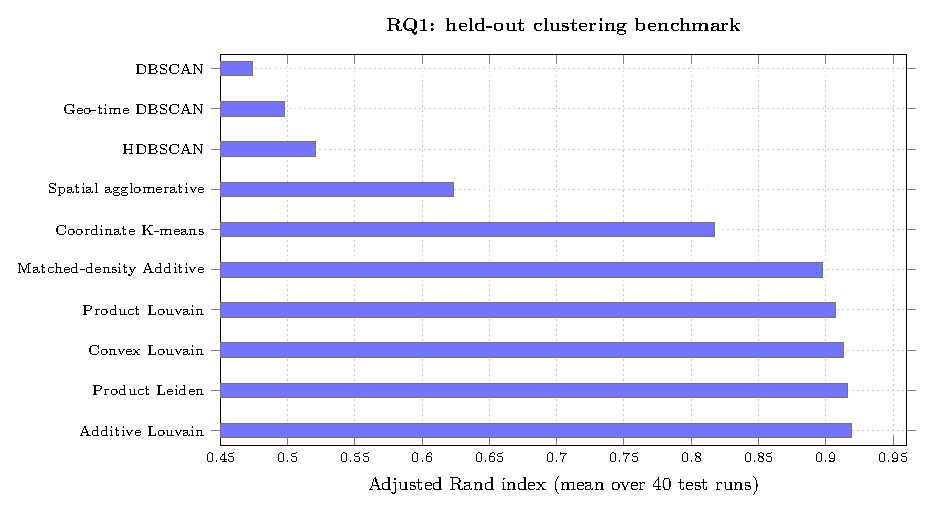
\includegraphics[width=\textwidth]{rq1_benchmark.pdf}
\caption{ARI trung bình RQ1 trên phần kiểm thử, sinh từ CSV tóm tắt chuẩn.}
\label{fig:rq1-benchmark}
\end{figure}

\begin{table}[t]
\centering\scriptsize
\caption{Kết quả chính RQ2/RQ3 từ các hiện vật Candidate-4.1. Hiệu ứng và
$p$ của RQ3 dùng 40 cặp seed sau khi lấy trung bình ba kịch bản nguồn lực
trong từng seed; phân tích 120 cặp seed--kịch bản ban đầu chỉ mang tính chẩn
\ đoán. Hiệu ứng ghép dương ưu tiên ứng viên sửa đổi; metric càng thấp càng
tốt dùng quy ước dấu định hướng của hiện vật.}
\label{tab:stress-results}
\begin{tabular}{llrr}
\toprule
Câu hỏi & Tương phản và metric & Hiệu ứng & Holm $p$\\
\midrule
RQ2 & NDCG@5 sửa đổi (tuyệt đối) & .6669 & --\\
    & NDCG@5 ngẫu nhiên (tuyệt đối) & .6763 & --\\
    & Sửa đổi $-$ cũ, NDCG@5 & +.0121 & .5882\\
    & Độ trôi ưu tiên bản sao chính xác & 0 & --\\
    & Độ trôi chiến dịch (sửa đổi tuyệt đối) & .1688 & --\\
    & Sửa đổi $-$ cũ, độ trôi chiến dịch & $-.1379$ & $9.1\times10^{-12}$\\
RQ3 & Sửa đổi $-$ cũ, thiệt hại tích & $-14.34$ & .563\\
    & Sửa đổi $-$ cũ, hạn chót tích & +.0188 & .247\\
    & Sửa đổi $-$ gần nhất, thiệt hại tích & $-69.88$ & $4.1\times10^{-5}$\\
    & Sửa đổi $-$ gần nhất, hạn chót tích & $-.1771$ & $1.3\times10^{-6}$\\
    & Tích $-$ cộng cùng mật độ, thiệt hại & $-18.34$ & .000168\\
\bottomrule
\end{tabular}
\end{table}

Đối với RQ2, NDCG@5 sửa đổi là .6669 (KTC [.6306,.7018]), Spearman là
-.0304 (KTC [-.1165,.0549]) và giao top năm là .285 (KTC [.2349,.3400]).
Điểm sửa đổi cao hơn điểm cũ .0121 trên NDCG@5, nhưng tương phản hiệu chỉnh
Holm không có ý nghĩa; nó thấp hơn điểm chỉ dân số (.6709) và ngẫu nhiên
(.6763). Nhân bản chính xác ở mức $2\times$, $5\times$ và $10\times$ tạo độ
trôi ưu tiên sửa đổi bằng 0. Một chiến dịch phối hợp độ tin cậy cao tạo độ
trôi .1688 và độ nâng ưu tiên giả .8828; độ trôi sửa đổi tệ hơn điểm cũ
$-.1379$ (Holm $p\approx9.1\times10^{-12}$). Vì vậy tính bị chặn không bảo
đảm độ tin cậy của xếp hạng.

\begin{figure}[t]
\centering
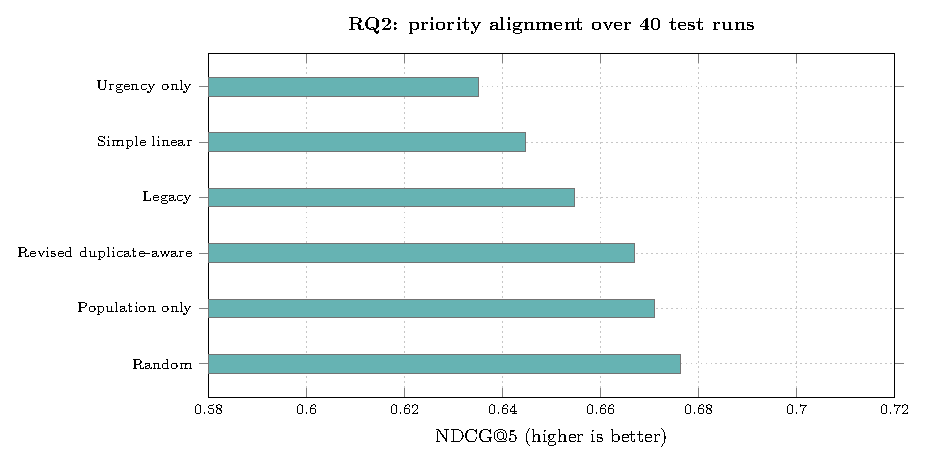
\includegraphics[width=\textwidth]{rq2_priority.pdf}
\caption{So sánh đồng chỉnh ưu tiên RQ2, sinh từ CSV tóm tắt Candidate-4.1.}
\label{fig:rq2-priority}
\end{figure}

Đối với RQ3, sau khi lấy trung bình ba kịch bản nguồn lực trong từng seed,
sửa đổi so với cũ trên phân hoạch tích có hiệu ứng thiệt hại $-14.34$
(Holm $p=.563$) và hiệu ứng hạn chót $+.0188$ (Holm $p=.247$), do đó chưa
xác lập được cải thiện tổng quát. Sửa đổi kém hơn đáng kể chiến lược gần nhất
trước ở cả thiệt hại (Holm $p=4.1\times10^{-5}$) và hạn chót (Holm
$p=1.3\times10^{-6}$). Dưới chính sách sửa đổi, tích cũng kém hơn cộng cùng
mật độ về thiệt hại (Holm $p=.000168$), và kém hơn oracle trên các kết quả
điều phối tương ứng. Các đích chỉ gồm giả và các lỗi tách, gộp dự đoán vì thế
lan truyền thành hệ quả tác nghiệp.

\begin{figure}[t]
\centering
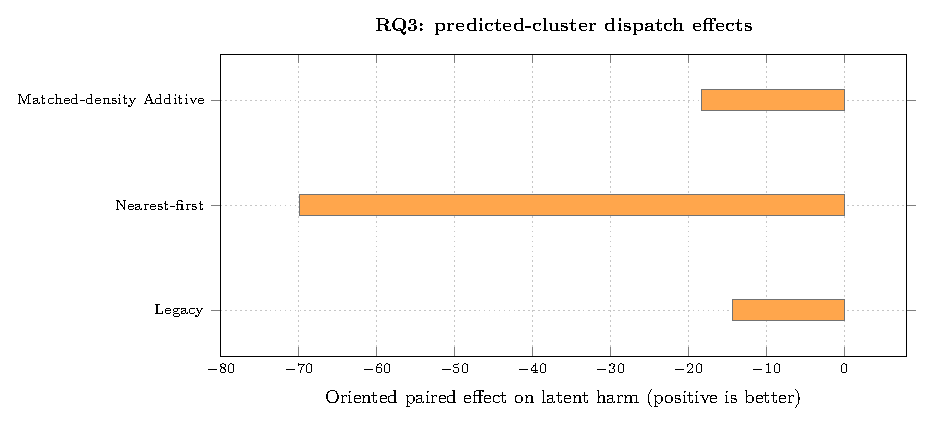
\includegraphics[width=\textwidth]{rq3_dispatch.pdf}
\caption{Hiệu ứng ghép RQ3 của phân hoạch tích trên thiệt hại ẩn, sinh từ
CSV so sánh điều phối theo seed; giá trị dương là cải thiện theo quy ước.}
\label{fig:rq3-dispatch}
\end{figure}

\subsection{Độ nhạy của các hằng số heuristic}
\label{sec:sensitivity}

Để đánh giá độ bền với các hằng số cố định trong $Q_i$ (Mục~2.1) và $P$
(Công thức~\ref{eq:priority}), chúng tôi định nghĩa phân tích độ nhạy cục bộ
từng biến một trên tác vụ xếp hạng Candidate-4.1. Mỗi hằng số hợp lệ được
nhiễu quanh giá trị tham chiếu trong khi các hằng số khác giữ nguyên, rồi
tính lại NDCG@5 trên cùng 40 seed kiểm thử. Các biến thể $\omega$ thay đổi
từng thành phần một lần và chuẩn hóa lại vector; $\mu$ bị giới hạn trong
khoảng hợp lệ của chính sách $[1,2]$. Lần chạy bị khóa đánh giá 21 cấu hình
(một baseline chung và hai hoặc ba mức thử cho mỗi hằng số) trên cùng 40 seed
giữ lại, tạo 840 quan sát cấp seed. Một hằng số được xem là ổn định nếu
metric trung bình thay đổi dưới 0.01 giữa các mức hợp lệ đã thử.

\begin{table}[t]
\centering\scriptsize
\caption{Độ nhạy từng biến một của NDCG@5 trung bình đối với các hằng số
heuristic Candidate-4.1. Mỗi khoảng là min--max trung bình trên các mức đã
thử, gồm cả mức tham chiếu, trên 40 seed kiểm thử. Mọi độ rộng đều dưới 0.01.}
\label{tab:sensitivity}
\resizebox{\textwidth}{!}{%
\begin{tabular}{lccc}
\toprule
Hằng số & Giá trị mặc định & Các mức thử & Khoảng metric\\
\midrule
$b_0$ (giao của $Q_i$) & $-0.20$ & $[-0.24,-0.16]$ & $[.6653,.6672]$\\
$b_1$ (trọng số ảnh) & $1.40$ & $[1.12,1.68]$ & $[.6669,.6687]$\\
$b_2$ (trọng số đối chứng) & $0.90$ & $[.72,1.08]$ & $[.6667,.6679]$\\
$\omega_E$ & $.34$ & thành phần $\times\{.8,1,1.2\}$, chuẩn hóa & $[.6663,.6714]$\\
$\omega_F$ & $.33$ & thành phần $\times\{.8,1,1.2\}$, chuẩn hóa & $[.6625,.6679]$\\
$\omega_N$ & $.33$ & thành phần $\times\{.8,1,1.2\}$, chuẩn hóa & $[.6663,.6697]$\\
$\mu$ (khuếch đại dễ tổn thương) & $2$ & $\{1.6,1.8,2.0\}$ & $[.6644,.6683]$\\
$s$ (bão hòa dễ tổn thương) & $10$ & $[8,12]$ & $[.6665,.6713]$\\
$N_{\rm ref}$ & $500$ & $[400,600]$ & $[.6669,.6669]$\\
$V_{\rm cap}$ & $50$ & $[40,60]$ & $[.6669,.6669]$\\
\bottomrule
\end{tabular}
}
\end{table}

\section{Thảo luận và các đe dọa đối với giá trị}

Kết quả tách biệt các biện pháp bảo đảm toán học khỏi tiện ích thực nghiệm.
Cổng tích cung cấp chặn cạnh hữu hạn trong miền ngưỡng dương, nhưng đường
ống tích được hiệu chỉnh độc lập không vượt qua phân cụm cộng. Ước lượng điểm
cùng mật độ đảo chiều hướng, song kiểm định đã hiệu chỉnh vẫn chưa kết luận.
Định lý đồ thị vì thế là tính chất định vị, không phải bằng chứng cho một
thành phần ưu tiên.

Điểm sửa đổi loại bỏ lạm phát do bản sao chính xác và giới hạn tính nhân bản,
nhưng không cho thấy ưu thế đồng chỉnh tổng quát. Thất bại trước chiến dịch
phối hợp đặc biệt quan trọng: đối thủ có thể tạo mẫu độ tin cậy cao, vẫn bị
chặn về số học nhưng làm xáo trộn xếp hạng. Kết quả điều phối xác nhận rằng
điểm bị chặn không thể thay thế một mục tiêu tác nghiệp đã được xác nhận; lỗi
phân cụm và các đích chỉ gồm giả được truyền sang lập lịch.

Phân tích độ nhạy cục bộ ổn định trên các khoảng đã thử: mọi hằng số có độ
rộng NDCG@5 trung bình dưới $0.01$ trên 40 seed giữ lại. Độ rộng lớn nhất là
của $\omega_F$ ($.00546$), trong khi đổi $V_{\rm cap}$ từ 40 lên 60 không
đổi trung bình ở độ chính xác được báo cáo. Các kết quả này chỉ hỗ trợ độ
ổn định số học trong lân cận đã thử; chúng không xác nhận các hằng số ngoài
các mức đó và không thay thế xác nhận chuyên gia.

Tất cả báo cáo, sự cố, tín hiệu liên quan và kết quả điều phối đều là tổng
hợp. RQ1 thay đổi seed trong generator 3.0.0, còn RQ2/RQ3 dùng bó
Candidate-4.1 riêng; không thử chuyển OOD có thay đổi cơ chế hay hiệu năng
thực địa. RQ1 không cung cấp kiểm thử thiếu dữ liệu thực nghiệm vì mọi báo
cáo được đánh giá đều có bốn thuộc tính lõi. Không có hội đồng chuyên gia
xác nhận trọng số ưu tiên, các chặn hay tiện ích. Nghiên cứu cũng không đo
độ chính xác trích xuất, độ trễ thiết bị, bộ nhớ, năng lượng, tính xác thực
nguồn gốc hay thiệt hại ngoài đời. Các hạn chế này loại trừ các tuyên bố về
chính sách hoặc triển khai.

\section{Kết luận}

Nghiên cứu thiết lập các chặn đồ thị có điều kiện và ghi nhận phân cụm cạnh
tranh trong cùng bộ sinh, tính bất biến với bản sao chính xác, cùng các kết
quả âm quan trọng đối với xếp hạng và điều phối. Nghiên cứu không thiết lập
đồng chỉnh xếp hạng, lợi ích điều phối, khả năng chống thông tin sai lệch,
tính hợp lệ chính sách hay mức sẵn sàng triển khai. Đóng góp là một ranh giới
kiểm thử sức chịu đựng có thể kiểm toán quanh các tuyên bố đó, không phải một
chính sách cứu hộ đã được xác nhận.

\section*{Khả dụng dữ liệu và mã nguồn}

Bản ghi hiện vật đi kèm chứa manifest của hai bộ dữ liệu, notebook chuẩn,
lưới hiệu chỉnh, cấu hình được chọn, kết quả kiểm thử từng lần chạy, các so
sánh ghép, phân tích lại RQ3 theo cấp seed và tập lệnh sinh hình xác định.
Các hình công bố được sinh từ các CSV kết quả; mọi con số báo cáo đều gắn với
một dòng CSV được chấp nhận và siêu dữ liệu bộ sinh/cấu hình được ghi lại.
Các snapshot neo thô từ nguồn upstream không được phân phối lại trong hiện
vật; tài liệu bên thứ ba vẫn chịu điều khoản nguồn gốc và giấy phép riêng.

Hiện vật nghiên cứu có phiên bản được lưu trữ trên Zenodo
\cite{nguyen2026floodartifact} và tương ứng với
\href{https://github.com/ngthtrong/nckh2/releases/tag/v1.0.0}{GitHub Release
v1.0.0} tại commit
\href{https://github.com/ngthtrong/nckh2/commit/04e0f04a7376cbbb02a1a95ecb4e3147d56c575b}{\texttt{04e0f04}}.
Phiên bản phát triển vẫn có trên nhánh
\href{https://github.com/ngthtrong/nckh2/tree/clean}{\texttt{clean}}.
Lần chạy lại dùng commit bộ sinh
\href{https://github.com/ngthtrong/nckh2/commit/a6be3e988dad1aa442c8c8e158c2bba96b2b7fb9}{\texttt{a6be3e9}};
manifest RQ2 ghi SHA-256 cho mọi CSV được báo cáo, gồm hiện vật độ nhạy 840
dòng và bản tóm tắt 30 dòng. Mã gốc phát hành theo giấy phép MIT, còn bản
thảo, bảng, hình và hiện vật tổng hợp gốc phát hành theo CC BY 4.0. Các cấp
phép này không bao gồm Copernicus EMS, OpenStreetMap, WorldPop, mẫu
Springer/LaTeX và các tài liệu bên thứ ba khác; chúng vẫn giữ điều khoản gốc
và yêu cầu ghi công tương ứng.

\bibliographystyle{splncs04}
\bibliography{references}

\end{document}
